% !TEX program = pdflatex
% !TEX encoding = UTF-8 Unicode

\documentclass{beamer}
\usepackage[utf8]{inputenc}
\usepackage[T1]{fontenc}
\usepackage{lmodern}
\usepackage{amsmath,amssymb}
\usepackage{graphicx}
\usepackage{booktabs}
\usepackage{hyperref}
\usepackage{tikz}
\usepackage{xcolor}
\usetikzlibrary{arrows.meta, positioning, shapes.geometric, calc}

\usetheme{Madrid}
\usecolortheme{default}

\definecolor{darkblue}{RGB}{0,51,102}
\definecolor{lightblue}{RGB}{173,216,230}
\definecolor{darkgreen}{RGB}{0,100,0}
\definecolor{darkorange}{RGB}{180,80,0}
\setbeamercolor{structure}{fg=darkblue}

%------------------------------------------------------------
\title[BDH Searchless Chess --- Final]{Searchless Chess: Neural Position Evaluation Without Tree Search}
\subtitle{Final Presentation --- Big Data in Healthcare}
\author{Antoni Czapski}
\institute[AGH UST]{AGH University of Science and Technology}
\date{March 2026}

%------------------------------------------------------------
\begin{document}

%------------------------------------------------------------
\frame{\titlepage}

%==============================================================================
% SLIDE: Agenda
%==============================================================================
\begin{frame}
\frametitle{Agenda}
\tableofcontents
\end{frame}

\section{Problem \& Dataset}
\section{Models}
\section{Critical Bug --- Error Analysis}
\section{Results \& Ablation}
\section{Engineering}
\section{Conclusions}

%==============================================================================
% SLIDE 1 — Problem
%==============================================================================
\begin{frame}
\frametitle{Problem: Searchless Chess}

\begin{columns}
\column{0.55\textwidth}

\textbf{Input:} Chess board position (FEN)\\
\textbf{Output:} Score $\in [-1, 1]$ $= \tanh(\text{cp}/1000)$\\
\textbf{Task:} Supervised regression

\vspace{0.7em}
No minimax. No alpha-beta. No MCTS.\\
\alert{Pure neural pattern recognition.}

\vspace{0.7em}
\textbf{Evaluation:} 1200 rated Lichess puzzles\\
\quad$\rightarrow$ per-tier solve rate $\rightarrow$ \textbf{ELO estimate}

\vspace{0.7em}
\textbf{Goal:} Match/exceed reference ViT-S at 1817 ELO.

\column{0.45\textwidth}
\begin{block}{Reference Results (Grzyb, 2025)}
\footnotesize
\begin{tabular}{lrc}
\toprule
\textbf{Model} & \textbf{Params} & \textbf{ELO} \\
\midrule
ViT-M     & 9.5M  & 1960 \\
ResNet-XL & 24.7M & 1719 \\
ResNet-L  & 12.9M & 1711 \\
\textbf{ViT-S}     & \textbf{2.6M}  & \textbf{1817} \\
ResNet-M  & 2.3M  & 1515 \\
CNN       & 1.2M  & 1112 \\
\bottomrule
\end{tabular}

\vspace{0.3em}
{\tiny Trained on 316M positions. Dataset: CC BY 4.0.}
\end{block}
\end{columns}

\end{frame}

%==============================================================================
% SLIDE 2 — Dataset & EDA
%==============================================================================
\begin{frame}
\frametitle{Dataset \& Exploratory Data Analysis}

\begin{columns}
\column{0.5\textwidth}

\textbf{lichess-stockfish-normalized} (HuggingFace)
\vspace{0.3em}
\begin{tabular}{lr}
\toprule
\textbf{Split} & \textbf{Positions} \\
\midrule
Train & 45,000,000 \\
Val   & 2,500,000  \\
Test  & 2,500,000  \\
\midrule
\textbf{Total} & \textbf{50M} \\
\bottomrule
\end{tabular}

\vspace{0.5em}
\textbf{Encoding:} FEN $\rightarrow$ \texttt{8$\times$8$\times$12} uint8\\
{\footnotesize 12 channels = 6 piece types $\times$ 2 colors\\
Always from side-to-move's perspective}

\vspace{0.3em}
\textbf{Target:} $\tanh(\text{cp} / 1000) \in [-1, 1]$\\
\textbf{Storage:} $\sim$34 GB (train boards, uint8)

\column{0.5\textwidth}

\begin{block}{Key EDA Insights}
\footnotesize
\begin{itemize}
  \item Distribution: symmetric, mean $\approx 0.02$, std $\approx 0.38$
  \item $\sim$50\% white-to-move, $\sim$50\% black \\ \alert{$\Rightarrow$ critical for preprocessing!}
  \item $\sim$45\% middlegame, 35\% endgame
  \item $\sim$15\% decisive positions ($|\text{score}|>0.9$)
  \item ``Predict zero'' baseline: MSE $\approx 0.145$
  \item Puzzle ELO strongly correlates with playing strength
\end{itemize}
\end{block}

\vspace{0.3em}
{\footnotesize Full EDA: \texttt{report/eda/eda.md}}

\end{columns}

\end{frame}

%==============================================================================
% SLIDE 3 — Architecture overview
%==============================================================================
\begin{frame}
\frametitle{Four Architectures Explored}

\begin{center}
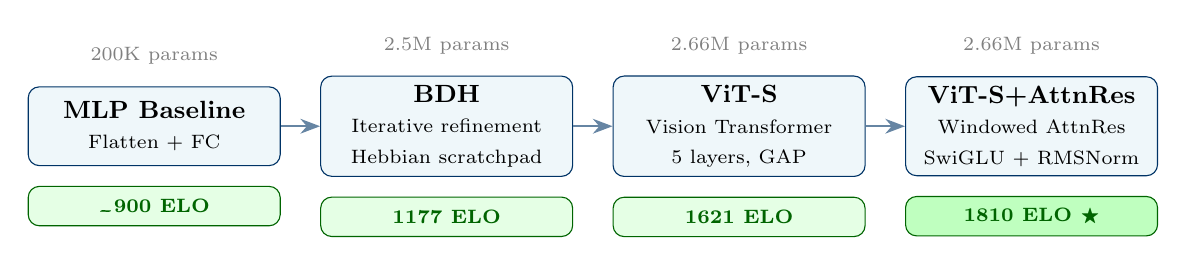
\begin{tikzpicture}[
  node distance=0.3cm and 0.5cm,
  arch/.style={rectangle, draw=darkblue, fill=lightblue!20, rounded corners,
               minimum height=1.0cm, minimum width=3.2cm, align=center, font=\small},
  elo/.style={rectangle, draw=darkgreen, fill=green!10, rounded corners,
              minimum height=0.5cm, minimum width=3.2cm, align=center, font=\scriptsize\bfseries, text=darkgreen},
  arrow/.style={-{Stealth[length=2.5mm]}, thick, darkblue!60}
]
\node[arch] (mlp) {\textbf{MLP Baseline}\\\scriptsize Flatten + FC};
\node[arch, right=of mlp] (bdh) {\textbf{BDH}\\\scriptsize Iterative refinement\\\scriptsize Hebbian scratchpad};
\node[arch, right=of bdh] (vit) {\textbf{ViT-S}\\\scriptsize Vision Transformer\\\scriptsize 5 layers, GAP};
\node[arch, right=of vit] (attn) {\textbf{ViT-S+AttnRes}\\\scriptsize Windowed AttnRes\\\scriptsize SwiGLU + RMSNorm};

\node[elo, below=0.25cm of mlp]  {\texttildelow 900 ELO};
\node[elo, below=0.25cm of bdh]  {1177 ELO};
\node[elo, below=0.25cm of vit]  {1621 ELO};
\node[elo, below=0.25cm of attn, fill=green!25] {\textbf{1810 ELO} $\bigstar$};

\draw[arrow] (mlp) -- (bdh);
\draw[arrow] (bdh) -- (vit);
\draw[arrow] (vit) -- (attn);

\node[above=0.15cm of mlp, font=\scriptsize, text=gray]  {200K params};
\node[above=0.15cm of bdh, font=\scriptsize, text=gray]  {2.5M params};
\node[above=0.15cm of vit, font=\scriptsize, text=gray]  {2.66M params};
\node[above=0.15cm of attn, font=\scriptsize, text=gray] {2.66M params};
\end{tikzpicture}
\end{center}

\vspace{0.5em}
\begin{center}
\begin{tabular}{lccc}
\toprule
& \textbf{Params} & \textbf{GPU-hours} & \textbf{ELO} \\
\midrule
MLP baseline    & 200K   & $<$1h   & $\sim$900 \\
BDH v4          & 2.5M   & $\sim$48h & 1177 \\
ViT-S v2        & 2.6M   & $\sim$17h & 1621 \\
\textbf{ViT-S+AttnRes} & \textbf{2.66M} & \textbf{$\sim$45h} & \textbf{1810} \\
\textit{Reference ViT-S} & \textit{2.6M} & \textit{$>$200h} & \textit{1817} \\
\bottomrule
\end{tabular}
\end{center}

\end{frame}

%==============================================================================
% SLIDE 4 — BDH Architecture
%==============================================================================
\begin{frame}
\frametitle{Model 1: BDH --- Iterative Value Refinement}

\begin{columns}
\column{0.52\textwidth}

\begin{center}
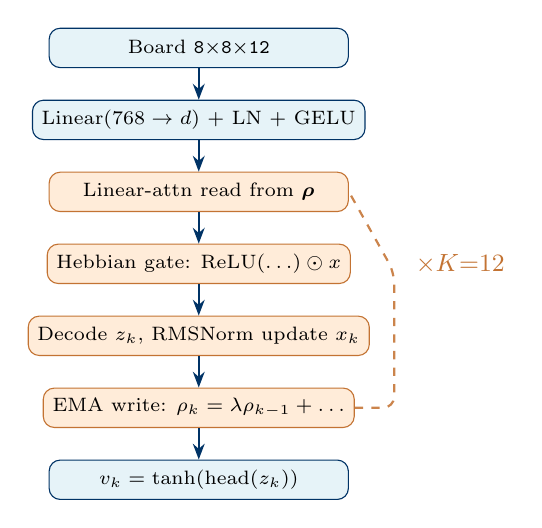
\begin{tikzpicture}[
  node distance=0.4cm,
  box/.style={rectangle, draw=darkblue, fill=lightblue!30, rounded corners,
              minimum height=0.5cm, minimum width=3.8cm, align=center, font=\scriptsize},
  recbox/.style={rectangle, draw=darkorange!80, fill=orange!15, rounded corners,
              minimum height=0.5cm, minimum width=3.8cm, align=center, font=\scriptsize},
  arrow/.style={-{Stealth[length=2mm]}, thick, darkblue},
  loopline/.style={thick, darkorange!70, dashed}
]
\node[box] (input) {Board \texttt{8$\times$8$\times$12}};
\node[box, below=of input] (embed) {Linear($768 \to d$) + LN + GELU};
\node[recbox, below=of embed] (a1) {Linear-attn read from $\boldsymbol{\rho}$};
\node[recbox, below=of a1] (a2) {Hebbian gate: $\mathrm{ReLU}(\ldots) \odot x$};
\node[recbox, below=of a2] (a3) {Decode $z_k$, RMSNorm update $x_k$};
\node[recbox, below=of a3] (a4) {EMA write: $\rho_k = \lambda\rho_{k-1} + \ldots$};
\node[box, below=of a4] (head) {$v_k = \tanh(\mathrm{head}(z_k))$};

\draw[arrow] (input)--(embed);
\draw[arrow] (embed)--(a1);
\draw[arrow] (a1)--(a2);
\draw[arrow] (a2)--(a3);
\draw[arrow] (a3)--(a4);
\draw[arrow] (a4)--(head);

\node[right=0.7cm of a2, font=\small\bfseries, text=darkorange!80] {$\times K{=}12$};
\draw[loopline, rounded corners] (a4.east)--++(0.5,0)--++(0,1.72)--(a1.east);
\end{tikzpicture}
\end{center}

\column{0.48\textwidth}

\textbf{Key idea:} Persistent synaptic state $\rho$ acts as a working-memory scratchpad across $K$ thinking steps.

\vspace{0.4em}
\textbf{Loss (deep supervision):}
{\scriptsize
$$\mathcal{L} = \underbrace{\mathrm{Huber}(v_K,y)}_{\text{final}} + 0.1\!\sum_{k<K}\!\underbrace{\mathrm{Huber}(v_k,y)}_{\text{intermediate}} + 0.01\!\underbrace{\sum_k (v_k - v_{k-1})^2}_{\text{stability}}$$
}

\vspace{0.2em}
\begin{block}{v1$\to$v4 Evolution}
\scriptsize
\begin{tabular}{ll}
\textbf{v1} & Sequence: 64 tokens (failed) \\
\textbf{v2} & Iterative: K=8, 500K data \\
\textbf{v3} & 50M data, NaN fix (bf16, RMSNorm) \\
\textbf{v4} & \alert{Score bug fixed}, ELO 1177 \\
\end{tabular}
\end{block}

\vspace{0.3em}
\textbf{Parameters:} 2.5M ($d$=256, $n_h$=8, $K$=12)\\
\textbf{VRAM:} $\sim$16 GB @ batch 2048 (A100)

\end{columns}

\end{frame}

%==============================================================================
% SLIDE 5 — ViT-S Architecture
%==============================================================================
\begin{frame}
\frametitle{Model 2: ViT-S --- Vision Transformer Small}

\begin{columns}
\column{0.52\textwidth}

\begin{center}
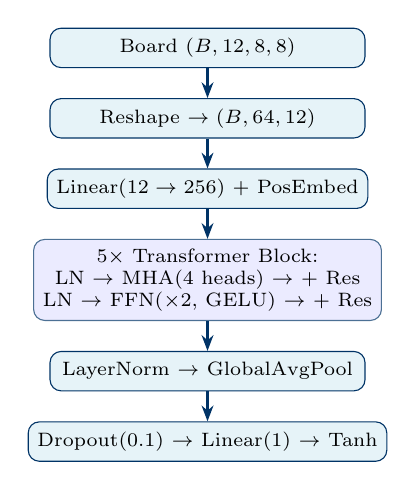
\begin{tikzpicture}[
  node distance=0.38cm,
  box/.style={rectangle, draw=darkblue, fill=lightblue!30, rounded corners,
              minimum height=0.5cm, minimum width=4.0cm, align=center, font=\scriptsize},
  tblock/.style={rectangle, draw=darkblue!70, fill=blue!8, rounded corners,
              minimum height=1.0cm, minimum width=4.0cm, align=center, font=\scriptsize},
  arrow/.style={-{Stealth[length=2mm]}, thick, darkblue}
]
\node[box] (input) {Board $(B,12,8,8)$};
\node[box, below=of input] (reshape) {Reshape $\to (B, 64, 12)$};
\node[box, below=of reshape] (proj) {Linear($12\to256$) + PosEmbed};
\node[tblock, below=of proj] (block) {5$\times$ Transformer Block:\\
  LN $\to$ MHA(4 heads) $\to$ + Res\\
  LN $\to$ FFN($\times$2, GELU) $\to$ + Res};
\node[box, below=of block] (gap) {LayerNorm $\to$ GlobalAvgPool};
\node[box, below=of gap] (head) {Dropout(0.1) $\to$ Linear(1) $\to$ Tanh};

\draw[arrow] (input)--(reshape);
\draw[arrow] (reshape)--(proj);
\draw[arrow] (proj)--(block);
\draw[arrow] (block)--(gap);
\draw[arrow] (gap)--(head);
\end{tikzpicture}
\end{center}

\column{0.48\textwidth}

\textbf{Faithful reimplementation} of the reference Keras model in PyTorch.

\vspace{0.4em}
\begin{block}{Key Design Choices}
\footnotesize
\begin{itemize}
  \item FFN ratio \textbf{2$\times$} (not standard 4$\times$)
  \item \textbf{Pre-norm} (LN before attention)
  \item \textbf{Global avg pool} --- no CLS token
  \item 64 patches of 12-dim (1 per square)
\end{itemize}
\end{block}

\vspace{0.4em}
\begin{block}{Training (v2 --- fixed)}
\footnotesize
\begin{tabular}{ll}
Params & 2,656,001 \\
Optimizer & AdamW \\
LR & $2\times10^{-4}$ (cosine) \\
Batch & 8192 \\
Precision & bf16 \\
Epochs & 30 (full) \\
GPU time & $\sim$17h \\
\alert{ELO} & \alert{1621} \\
\end{tabular}
\end{block}

\end{columns}

\end{frame}

%==============================================================================
% SLIDE 6 — CRITICAL BUG
%==============================================================================
\begin{frame}[fragile]
\frametitle{Critical Bug: Score Perspective Error}

\begin{alertblock}{Symptom}
Both BDH and ViT trained cleanly for 25--30 epochs, but achieved ELO~$\approx$~$-3500$ (worse than random).
\end{alertblock}

\vspace{0.4em}
\begin{columns}
\column{0.5\textwidth}

\begin{block}{Root Cause}
\footnotesize
HuggingFace dataset stores scores \textbf{from white's perspective}. Our encoding mirrors the board for black-to-move (\texttt{always\_white\_perspective=True}).\\[0.4em]
The score was \textbf{never flipped} for black:\\[0.3em]
\begin{tabular}{lll}
\toprule
Position & Board & Score \\
\midrule
White to move & correct & correct \\
Black to move & mirrored & \alert{wrong sign} \\
\bottomrule
\end{tabular}\\[0.4em]
$\Rightarrow$ \textbf{50\% of labels inverted}. Model learns to predict $\approx 0$ to minimize MSE.
\end{block}

\column{0.5\textwidth}

\begin{block}{The Fix (one line)}
\scriptsize
\begin{verbatim}
sign = 1.0 if " w " in fen else -1.0
score = sign * normalize_cp(raw_cp)
\end{verbatim}
\end{block}

\vspace{0.4em}
\begin{block}{Impact}
\footnotesize
\begin{tabular}{lrr}
\toprule
\textbf{Model} & \textbf{Before} & \textbf{After} \\
\midrule
ViT-S ELO   & $-3488$ & \textbf{1621}  \\
BDH ELO     & $-2969$ & \textbf{1177}  \\
ViT-S acc   & 5.3\%   & \textbf{45.1\%} \\
ViT val MSE & 0.1525  & \textbf{0.0347} \\
\bottomrule
\end{tabular}
\end{block}

\vspace{0.2em}
\alert{Lesson: Validate preprocessing end-to-end with a sanity benchmark before training at scale.}

\end{columns}

\end{frame}

%==============================================================================
% SLIDE 7 — AttnRes
%==============================================================================
\begin{frame}
\frametitle{Model 3: ViT-S + Attention Residuals}

\begin{columns}
\column{0.5\textwidth}

\begin{block}{Standard Residual (ViT-S)}
\small
$$h_l = h_{l-1} + f_l(\mathrm{LN}(h_{l-1}))$$
\vspace{-0.4em}
{\footnotesize Fixed equal-weight sum of all previous outputs.}
\end{block}

\vspace{0.4em}
\begin{block}{Attention Residual (Kimi, 2025)}
\small
$$h_l = \sum_{i=0}^{l-1} \alpha_{i \to l}\, v_i, \quad \alpha = \mathrm{softmax}_{\mathrm{depth}}(w_l^\top \mathrm{RMSNorm}(v_i))$$
\vspace{-0.4em}
{\footnotesize Learned pseudo-query $w_l$ selects the most useful earlier layer. Sources: embedding + all previous sublayer outputs.}
\end{block}

\vspace{0.4em}
\textbf{Windowed (W=3):} Only last 3 depth sources.\\
{\footnotesize Full AttnRes $\Rightarrow$ CUDA OOM on A100-40GB}

\column{0.5\textwidth}

\begin{block}{Changes vs base ViT-S}
\footnotesize
\begin{tabular}{lll}
\toprule
\textbf{Component} & \textbf{ViT-S} & \textbf{+AttnRes} \\
\midrule
Residuals  & Fixed sum    & \alert{Learned mix} \\
FFN        & GELU $\times$2 & \alert{SwiGLU $\times$3} \\
Norm       & LayerNorm    & \alert{RMSNorm} \\
Params     & 2.656M       & 2.665M (+0.3\%) \\
\bottomrule
\end{tabular}
\end{block}

\vspace{0.4em}
\begin{block}{Result}
\footnotesize
\begin{tabular}{lrr}
\toprule
& \textbf{ViT-S} & \textbf{+AttnRes} \\
\midrule
ELO          & 1621    & \textbf{1810} \\
Puzzle acc   & 45.1\%  & \textbf{53.0\%} \\
Best val MSE & 0.03470 & \textbf{0.03379} \\
Epochs to best & 27   & \textbf{14} \\
\midrule
$\Delta$ & \multicolumn{2}{c}{\textbf{+189 ELO, +7.9 pp, $-$0.3\% loss}} \\
\bottomrule
\end{tabular}
\end{block}

\end{columns}

\end{frame}

%==============================================================================
% SLIDE 8 — Ablation: per-tier puzzle accuracy
%==============================================================================
\begin{frame}
\frametitle{Ablation Study: Per-Tier Puzzle Accuracy}

\begin{center}
\footnotesize
\begin{tabular}{lrrrr}
\toprule
\textbf{Puzzle Tier (ELO)} & \textbf{BDH v4} & \textbf{ViT-S v2} & \textbf{ViT+AttnRes} & \textbf{Ref ViT-S} \\
\midrule
0--500     & 82\%  & 87\%  & \textbf{89\%} & --- \\
500--750   & 71\%  & 87\%  & \textbf{96\%} & --- \\
750--1000  & 62\%  & 77\%  & \textbf{87\%} & --- \\
1000--1250 & 43\%  & 73\%  & \textbf{78\%} & --- \\
1250--1500 & 38\%  & 70\%  & \textbf{79\%} & --- \\
1500--1750 & 23\%  & 58\%  & \textbf{66\%} & --- \\
1750--2000 & 21\%  & 37\%  & \textbf{46\%} & --- \\
2000--2250 & 15\%  & 31\%  & \textbf{33\%} & --- \\
2250--2500 & 11\%  & 9\%   & \textbf{15\%} & --- \\
2500--2750 & 4\%   & 7\%   & \textbf{9\%}  & --- \\
2750--3000 & 1\%   & 4\%   & 2\%   & --- \\
3000--3250 & 1\%   & 2\%   & \textbf{3\%}  & --- \\
\midrule
\textbf{Overall acc} & 31.0\% & 45.1\% & \textbf{53.0\%} & --- \\
\textbf{ELO}         & 1177   & 1621   & \textbf{1810}   & \textbf{1817} \\
\bottomrule
\end{tabular}
\end{center}

\vspace{0.3em}
\begin{itemize}
  \item AttnRes improves most in mid-range (750--2000 ELO): +9--17 pp --- learned depth mixing helps positional evaluation.
  \item All models struggle above 2500 ELO: requires multi-move tactical calculation (no tree search).
  \item \alert{Only 7 ELO below reference} despite using 6.3$\times$ less data (50M vs 316M).
\end{itemize}

\end{frame}

%==============================================================================
% SLIDE 9 — All experiments
%==============================================================================
\begin{frame}
\frametitle{Full Experiment Log --- 10 Runs}

\begin{center}
\scriptsize
\begin{tabular}{llrrrrr}
\toprule
\textbf{\#} & \textbf{Experiment} & \textbf{Fix?} & \textbf{Params} & \textbf{GPU-h} & \textbf{Acc} & \textbf{ELO} \\
\midrule
1 & BDH v1 (sequence, local) & \texttimes & 796K  & $<$1h  & 0.5\%  & --- \\
2 & BDH v2 (iterative, local) & \texttimes & 682K  & $<$1h  & 0.8\%  & --- \\
3 & BDH v3 (50M, A100)        & \texttimes & 2.5M  & 34h    & 5.8\%  & $-$2969 \\
4 & ViT-S sanity check        & \texttimes & 2.6M  & 31h    & 5.3\%  & $-$3488 \\
\midrule
\multicolumn{7}{c}{\textit{\alert{Score perspective bug discovered \& fixed}}} \\
\midrule
5 & \textbf{ViT-S v2 (fixed)} & \checkmark & 2.6M  & 17h    & 45.1\% & \textbf{1621} \\
6 & \textbf{BDH v4 (fixed)}   & \checkmark & 2.5M  & 48h    & 31.0\% & \textbf{1177} \\
7 & ViT+AttnRes (14 ep)        & \checkmark & 2.66M & 24h    & 49.3\% & 1729 \\
8 & \textbf{ViT+AttnRes (27 ep)} & \checkmark & 2.66M & 45h  & \textbf{53.0\%} & \textbf{1810} \\
\midrule
  & \textit{Reference ViT-S}   & \checkmark & 2.6M  & $>$200h & --- & 1817 \\
\bottomrule
\end{tabular}
\end{center}

\vspace{0.2em}
\begin{block}{Takeaways}
\footnotesize
\begin{enumerate}
  \item Preprocessing bug (row 3--4) is far more damaging than any architecture choice.
  \item ViT-S beats BDH by 444 ELO on identical data --- spatial attention $>$ flattened recurrence.
  \item AttnRes adds +189 ELO over ViT-S with only +0.3\% parameters.
  \item We match reference with 6.3$\times$ less data and $\sim$4$\times$ less compute.
\end{enumerate}
\end{block}

\end{frame}

%==============================================================================
% SLIDE 10 — Engineering & DevOps
%==============================================================================
\begin{frame}[fragile]
\frametitle{Engineering \& DevOps}

\begin{columns}
\column{0.5\textwidth}

\begin{block}{\texttt{uv} + Config-driven training}
\scriptsize
\begin{verbatim}
uv sync --all-extras
uv run python scripts/train.py \
    --config configs/train_vit_attnres_a100.yaml
# smoke test (CPU, synthetic):
uv run python scripts/train.py \
    --config configs/smoke/vit_smoke.yaml \
    --smoke-test
\end{verbatim}
\end{block}

\begin{block}{Tests (104 tests, all passing)}
\footnotesize
\begin{itemize}
  \item \texttt{test\_config\_loads.py} --- all 8 YAML configs
  \item \texttt{test\_board\_encoding.py} --- FEN, normalize\_cp
  \item \texttt{test\_model\_forward\_vit.py} --- all 4 architectures
  \item \texttt{test\_lightning\_smoke\_train.py} --- fast\_dev\_run
  \item \texttt{test\_evaluation\_smoke.py} --- puzzle pipeline
\end{itemize}
\end{block}

\column{0.5\textwidth}

\begin{block}{CI/CD (GitHub Actions)}
\footnotesize
\begin{tabular}{ll}
\toprule
\textbf{Step} & \textbf{Tool} \\
\midrule
Deps install & \texttt{uv sync --all-extras} \\
Lint         & \texttt{ruff check} \\
Compile      & \texttt{python -m compileall} \\
Tests        & \texttt{pytest} (104 tests) \\
\bottomrule
\end{tabular}\\[0.2em]
\footnotesize On every push \& PR to \texttt{main}.
\end{block}

\begin{block}{Reproducibility}
\footnotesize
\begin{itemize}
  \item \texttt{uv.lock} --- 189 packages pinned
  \item Seeds: \texttt{seed\_everything(42)}
  \item Fixed 90/5/5 splits (seed=42)
  \item Checkpoint resume (optimizer + scheduler)
  \item W\&B: 10 logged experiments
\end{itemize}
\end{block}

\end{columns}

\end{frame}

%==============================================================================
% SLIDE 11 — Error Analysis: Where models fail
%==============================================================================
\begin{frame}
\frametitle{Error Analysis: Where Models Fail}

\begin{columns}
\column{0.5\textwidth}

\textbf{1. Score perspective bug (fixed)}\\
{\footnotesize 50\% label inversion $\to$ model predicts $\approx 0$ $\to$ $-3488$ ELO. Invisible during training (smooth loss curves, reasonable MAE). Only detectable via puzzle benchmark.}

\vspace{0.5em}
\textbf{2. High-ELO tactical puzzles}\\
{\footnotesize All models fail above 2500 ELO. Puzzles at that level require 3--5 move combinations. Without search, the model can only evaluate positions, not plan sequences.}

\vspace{0.5em}
\textbf{3. BDH overfits more than ViT}\\
{\footnotesize BDH v4: 26.5\% train-val gap. ViT-S: 5.2\%. Shared-weight 12-step loop memorizes training positions without proportional generalization.}

\column{0.5\textwidth}

\textbf{4. NaN divergence (BDH v3, fixed)}\\
{\footnotesize Unbounded ReLU + residual growth $\to$ fp16 overflow. Fixed with: RMSNorm on neurons, normalized $\rho$ writes, bf16 precision.}

\vspace{0.5em}
\textbf{5. CUDA OOM (full AttnRes)}\\
{\footnotesize Full AttnRes keeps all 11 depth sources live in the compute graph. At batch 4096: 30--40 GB VRAM $\to$ OOM on A100-40GB. Fixed with Windowed AttnRes (W=3).}

\vspace{0.5em}
\begin{alertblock}{Key Lesson}
\footnotesize
All critical failures (score bug, NaN, OOM) were \textbf{infrastructure / data problems}, not model design issues. Robust pipelines matter more than novel architectures.
\end{alertblock}

\end{columns}

\end{frame}

%==============================================================================
% SLIDE 12 — Conclusions
%==============================================================================
\begin{frame}
\frametitle{Conclusions}

\begin{columns}
\column{0.55\textwidth}

\begin{block}{Key Findings}
\footnotesize
\begin{enumerate}
  \item \textbf{AttnRes works:} +189 ELO over ViT-S with +0.3\% params. Learned depth mixing $>$ fixed residuals.
  \item \textbf{Label quality dominates:} Score bug cost 5000+ ELO. Validate preprocessing with real benchmarks, not just loss curves.
  \item \textbf{ViT $>$ BDH:} 444 ELO advantage on identical data. Spatial attention captures chess structure better than flattened recurrent processing.
  \item \textbf{Reference result reproduced:} \alert{1810 ELO} (ref: 1817) with 6.3$\times$ less data and 4$\times$ less compute.
  \item \textbf{Data scale is the bottleneck:} 500K $\to$ 50M was transformative. 50M $\to$ 316M would likely close the 7-point gap.
\end{enumerate}
\end{block}

\column{0.45\textwidth}

\begin{block}{Limitations}
\footnotesize
\begin{itemize}
  \item No tree search --- fails on deep tactics ($>$2500 ELO)
  \item Simplified encoding (no castling, en passant, move history)
  \item 6.3$\times$ less data than reference
  \item Windowed AttnRes (W=3), not full depth retrieval
\end{itemize}
\end{block}

\begin{block}{Future Work}
\footnotesize
\begin{itemize}
  \item Scale to 316M positions
  \item Add policy head (move probabilities)
  \item Adaptive halting for BDH (variable $K$)
  \item Gradient checkpointing for full AttnRes
  \item Richer encoding: castling, en passant
\end{itemize}
\end{block}

\end{columns}

\end{frame}

%==============================================================================
% SLIDE 13 — Summary
%==============================================================================
\begin{frame}
\frametitle{Summary}

\begin{center}
\large
\begin{tabular}{rl}
\textbf{Problem}      & Searchless chess position evaluation \\[0.4em]
\textbf{Dataset}      & 50M positions (HuggingFace, CC BY 4.0) \\[0.4em]
\textbf{Architectures}& MLP $\to$ BDH $\to$ ViT-S $\to$ \alert{ViT-S+AttnRes} \\[0.4em]
\textbf{Best result}  & \alert{1810 ELO} (reference: 1817, $\Delta = -7$) \\[0.4em]
\textbf{Key finding}  & Score bug fixed: $-3488 \to 1810$ ELO \\[0.4em]
\textbf{Experiments}  & 10 runs, $\sim$200 GPU-hours total (A100) \\[0.4em]
\textbf{Engineering}  & \texttt{uv} + Lightning + CI + 104 tests + W\&B \\[0.4em]
\textbf{Compute}      & 6.3$\times$ less data, 4$\times$ less compute vs ref \\
\end{tabular}
\end{center}

\vspace{1em}
\begin{center}
\large
\textbf{Repository:} \url{github.com/antoniczapski/searchless-chess}\\[0.5em]
\Large \textbf{Questions?}
\end{center}

\end{frame}

\end{document}
